\documentclass{eplDoc}
\usepackage{placeins}


\newcommand{\docType}	{Assignment 1 : Corpus Processing}
\newcommand{\docDate}	{01/03/2012}
\newcommand{\docAuthor}	{gr10 : Mulders Corentin, Pelsser François}
\newcommand{\courseCode}{LINGI2263}
\newcommand{\courseName}{Computational linguistics}
\usepackage{syntax}
\begin{document}
\maketitle
\newpage
\addtocounter{section}{1}

\section{Preprocessing}
To tokenize the files we had to determine where to split the sentences in words and wich types of expressions should be replaced by a token representing the type. \\ 
For slitting the tokens we simply used the whitespace as a separator as well as special characters that we didn't include in our types definitions. With the exception of the special characters "-" and "'" wich can appear inside some tokens that we didn't wish to split. \\ 
We also added markers for start and end of sentences. The start of sentences where placed before capitalized words followed by any sequence of tokens finishing by a dot or a newline. The end of sentences where then placed after any dot followed by either a start of sentence, a newline or the end of the string.
\subsection{Mapping expressions to types}
We replaced some types of expressions by aliases : 
\begin{description}
	\item[email] replaces any email
	\item[date] replaces the dates
	\item[kikoo] replaces words such as "xoXOxo" or any variation.
	\item[smiley] replaces any smiley
	\item[math] replaces mathematical expressions
	\item[punctuationfreak] replaces multiple punctuation marks.
	\item[repeatedchars] replaces any word containing a letter repeated 3 or more times in a row.
	\item[weirdcaps] replaces words with a least a non capitalized character followed by a capitalized one.
\end{description}

We also replaced occurences of "'s" by "is" and of "'m" by "am".
\subsection{Most frequent tokens}
After tokenizing the corpus (composed of the training files for both male and female blogs) the total number of tokens retrieved in the lexicon is  57698  distinct tokens.  \\ 
Here are the top 20 most frequent tokens types extracted from the corpus. We removed the markers <s> and </s> used to represent respectively the beginning and the end of a sentence from this top list. They were in the top 2 postiions and weren't really interesting. \\ 
\begin{center}
		\begin{tabular}{|l|c|}
			\hline
			token & frenquency \\
			\hline
			the  &  34631 \\ 
			to  &  22906 \\ 
			and  &  21281 \\ 
			a  &  19722 \\ 
			of  &  18168 \\ 
			I  &  16620 \\ 
			is  &  16436 \\ 
			in  &  11903 \\ 
			that  &  9428 \\ 
			for  &  7512 \\ 
			it  &  7179 \\ 
			on  &  6184 \\ 
			my  &  5854 \\ 
			was  &  5843 \\ 
			with  &  5705 \\ 
			you  &  5656 \\ 
			have  &  4692 \\ 
			this  &  4468 \\ 
			be  &  4186 \\ 
			as  &  4157 \\ 
			\hline
		\end{tabular}
\end{center}
 \ \\ 
We can see that the word "the" is the most frequent one as expected. 

\section{Word and N-gram counts}
Here is the graph of the number of unigrams, bigrams and trigrams for each frequency :
\FloatBarrier
\begin{figure}%
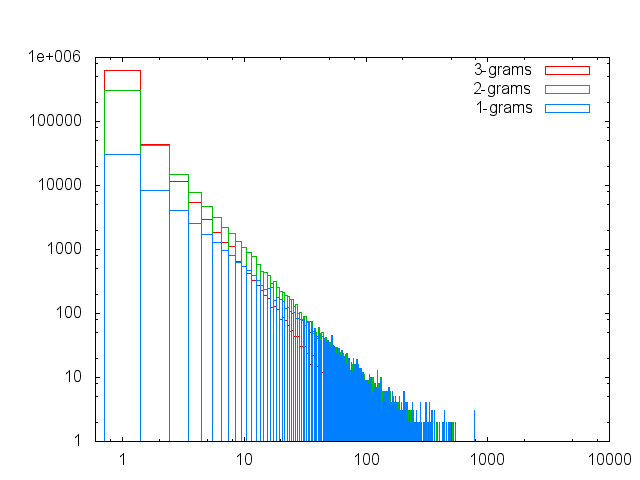
\includegraphics[width=\columnwidth]{ngramsplot.png}%
\caption{}%
\label{}%
\end{figure}
\FloatBarrier

We can see the unigrams histogram in blue and it is linear in log-log scale so Zipf's law is respected. \\ 
The same seems to be true for bigrams and trigrams. 

\section{N-gram estimation}

\section{Categorization of blog messages per gender}

\end{document}
